\chapter{Client Software} \label{sec:clientsw}

With the communication protocol clearly defined in \cref{sec:tinyframe,sec:units_overview}, and \cref{sec:wireless} for the wireless gateway, the implementation of client libraries is relatively straightforward. Two have been developed as a proof-of-concept, in languages C and Python.

\section{General Library Structure}

The structure of a GEX client library is in all cases similar:

\begin{itemize}
    \item \textbf{USB or serial port access}

        This is the only platform-dependent part of the library. Unix-based systems provide a standardized POSIX API to configure the serial port. A raw access to \gls{USB} endpoints is possible using the libUSB C library. Access to the serial port or \gls{USB} from C on MS Windows has not been investigated, but should be possible using proprietary APIs.

        Accessing the serial port or \gls{USB} endpoints from Python is more straightforward thanks to the cross platform libraries \textit{PySerial} and \textit{PyUSB}.

    \item \textbf{TinyFrame implementation}

        The \textit{TinyFrame} protocol library can be used directly in desktop C applications, and it has been re-implemented in Python and other languages.

    \item \textbf{Higher-level GEX logic}

        The host side of the communication protocol described in \cref{sec:tinyframe} should be implemented as a part of the library. This includes the reading and writing of configuration files, unit list read-out, command payload building, and asynchronous event parsing.

        Additional utilities may be defined on top of this basic protocol support for the command API of different GEX units, as described in \cref{sec:units_overview}. Those unit-specific ``drivers'' are available in the provided Python library.
\end{itemize}

\section{Python Library}

The Python GEX library implements both a serial port access and raw access to \gls{USB} endpoints. Its development has been prioritized over the C library because of its potential to integrate with MATLAB, and because it promises to be the most convenient method to interact with GEX thanks to the ease-of-use that comes with the Python syntax. This library provides a high level \gls{API} above the individual unit types, removing the burden of building and parsing of the binary command payloads from the user.

The library is composed of a \textit{transport} class, the core class \mono{gex.Client}, and unit classes (e.g., \mono{gex.I2C} or \mono{gex.SPI}). 

\noindent
Three transport implementations have been developed:

\begin{itemize}
    \item \mono{gex.TrxSerialSync} -- virtual serial port access with polling for a response

    \item \mono{gex.TrxSerialThread} -- virtual serial port access with a polling thread and semaphore-based notifications

    \item \mono{gex.TrxRawUSB} -- similar to \mono{gex.TrxSerialThread}, but using raw USB endpoint access
\end{itemize}

To use the wireless gateway, wrap either low-level transport in \mono{gex.DongleAdapter}. The adapter configures the gateway and converts the regular protocol to the right format.

\begin{pythoncode}
# Gateway connection example
transport = gex.DongleAdapter(gex.TrxRawUSB(remote=True), slave=42)
client = gex.Client(transport)
# ...
client.close()
\end{pythoncode}

\subsection{Example Python Script} \label{sec:ex_python_script}

An example Python program displaying a test pattern on a \gls{LED} matrix using the \gls{I2C}-connected driver chip IS31FL3730 is presented in \cref{lst:py_api} as an illustration of the library usage. A photo of the produced \gls{LED} pattern can be seen in \cref{fig:pydemo}.

\begin{listing}
	\begin{pythoncode}
#!/bin/env python3
# The I2C unit, called 'i2c', is configured to use PB6 and PB7
import gex
with gex.Client(gex.TrxRawUSB()) as client:
    bus = gex.I2C(client, 'i2c')
    addr = 0x61
    bus.write_reg(addr, 0x00, 0b00011000) # dual matrix
    bus.write_reg(addr, 0x0D, 0b00001110) # 34 mA
    bus.write_reg(addr, 0x19, 64) # set brightness
    # matrix 1
    bus.write_reg(addr, 0x01, [
        0xAA, 0x55, 0xAA, 0x55,
        0xAA, 0x55, 0xAA, 0x55
    ])
    # matrix 2
    bus.write_reg(addr, 0x0E, [
        0xFF, 0x00, 0xFF, 0x00,
        0xFF, 0x00, 0xFF, 0x00
    ])
    # update display
    bus.write_reg(addr, 0x0C, 0x01)
	\end{pythoncode}
	\caption{\label{lst:py_api} An example Python program using the GEX client library}
\end{listing}

\begin{figure}
	\centering
	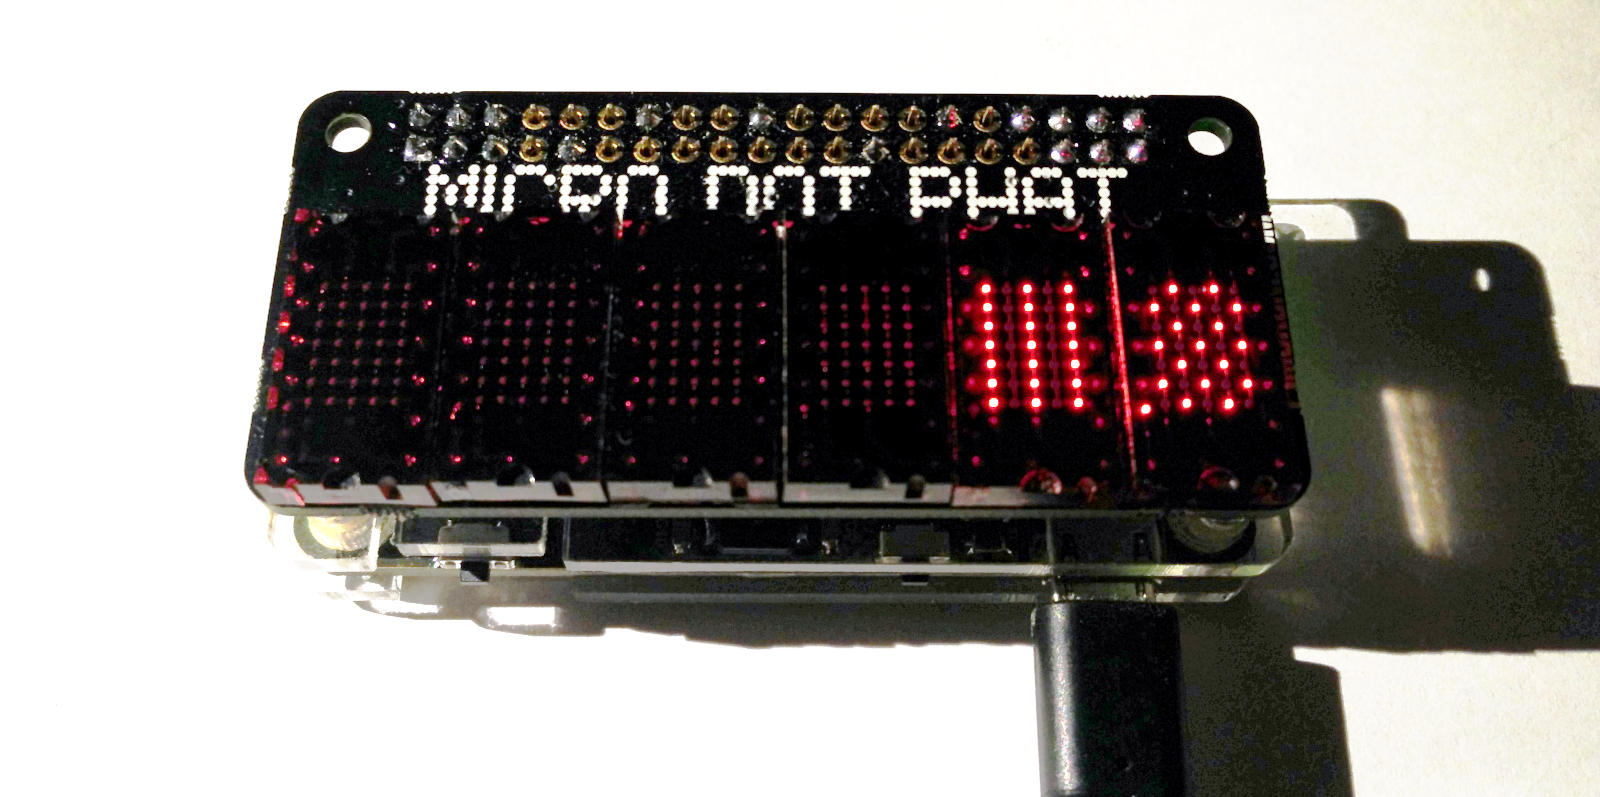
\includegraphics[width=.7\textwidth] {img/phatmtx.jpg}
	\caption[GEX Zero with the Micro Dot pHAT add-on board]{\label{fig:pydemo}GEX Zero with the Micro Dot pHAT add-on board, showing a test pattern defined in a Python script}
\end{figure}

First, a client instance is created, receiving the transport as an argument. We use a \mono{with} block in the example to ensure the transport is safely closed before the program ends, even if that happens due to an exception; this is similar to the \mono{try-finally} pattern, but the de-initialization is done automatically. The client (and subsequently the transport) can be closed manually by calling its \mono{.close()} method. Inside the \mono{with} block, the script proceeds to create unit handles and use them to perform the desired task, in our case a communication with the \gls{LED} matrix driver over the \gls{I2C} bus.

\section{MATLAB integration}

The Python library can be accessed from MATLAB scripts thanks to MATLAB's two-way Python integration~\cite{matlabpy}. Controlling GEX from MATLAB may be useful when additional processing is required, e.g., with data from the \gls{ADC}; however, in many cases, an open source alternative native to Python exists that could be used for the same purpose, such as the NumPy and SciPy libraries~\cite{numpyscipy}.

The example in \cref{lst:matlab_api} (and \cref{fig:matlabpic}) demonstrates the use of MATLAB to calculate the frequency spectrum of an analog signal captured with GEX. The syntax needed to use the serial port transport (instead of a raw access to USB endpoints) is shown in a comment.

\begin{listing}
	\begin{matlabcode}
	% The ADC unit, called 'adc', is configured to use PA1 as Channel 0
	
	%trx = py.gex.TrxSerialThread(pyargs('port', '/dev/ttyUSB1', ...
	%                                    'baud', 115200));
	trx = py.gex.TrxRawUSB();
	client = py.gex.Client(trx);
	adc = py.gex.ADC(client, 'adc');
	
	L = 1000; Fs = 1000;
	adc.set_sample_rate(uint32(Fs)); % casting to unsigned integer
	data = adc.capture(uint32(L));
	data = double(py.array.array('f',data)); % numpy array to matlab format
	
	Y = fft(data);
	P2 = abs(Y/L);
	P1 = P2(1:L/2+1);
	P1(2:end-1) = 2*P1(2:end-1);
	f = Fs*(0:(L/2))/L;
	
	plot(f,P1)
	client.close()
	\end{matlabcode}
	\caption{\label{lst:matlab_api} Calling the Python GEX library from a MATLAB script}
\end{listing}

\begin{figure}
	\centering
	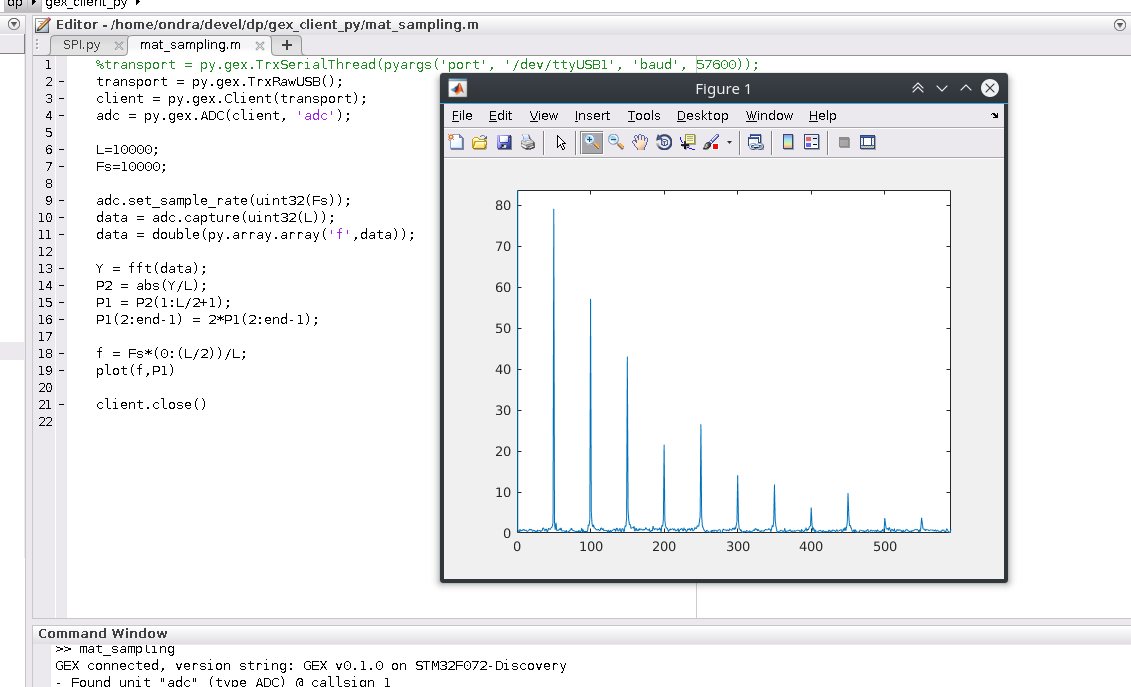
\includegraphics[width=\textwidth]{img/matlab-fft.png}
	\caption{A demonstration of the MATLAB/Python integration}
	\label{fig:matlabpic}
\end{figure}

\section{C Library}

The C library is more simplistic than the Python one; it supports only the serial port transport (\gls{UART} or \gls{CDCACM}) and does not implement asynchronous polling or the unit support drivers. The implemented features---the transport, a basic protocol handler, and payload building and parsing utilities---are sufficient for most applications, though less convenient than the Python library.

This low-level library is intended for applications where the performance of the Python implementation is insufficient, or where an integration with existing C code is required. The full \gls{API} can be found in the library header files. A C version of the example Python script shown above, controlling an \gls{LED} matrix driver, is presented in \cref{lst:c_api_full}. The payloads in this example are represented as binary strings for simplicity. Two better methods of payload construction are available: using C structs, or taking advantage of the Payload Builder utility (bundled with TinyFrame).

\begin{listing}
	\begin{ccode}
	#include <signal.h>
	#include <assert.h>
	#include "gex.h"
			
	void main(void)
	{
	    // Initialize GEX and the I2C unit handle
	    GexClient *gex = GEX_Init("/dev/ttyACM0", 200);
	    assert(NULL != gex);        
	    GexUnit *bus = GEX_GetUnit(gex, "i2c", "I2C");
	    assert(NULL != bus);	    	    
	    // Configure the matrix driver
	    GEX_Send(bus, 2, (uint8_t*) "\x61\x00\x00\x18", 4);
	    GEX_Send(bus, 2, (uint8_t*) "\x61\x00\x0d\x0e", 4);
	    GEX_Send(bus, 2, (uint8_t*) "\x61\x00\x19\x40", 4);	    
	    // Load data
	    GEX_Send(bus, 2, (uint8_t*) "\x61\x00\x01"
	                                "\xAA\x55\xAA\x55\xAA\x55\xAA\x55", 11);
	    GEX_Send(bus, 2, (uint8_t*) "\x61\x00\x0e"
	                                "\xFF\x00\xFF\x00\xFF\x00\xFF\x00", 11);
	    // Update display
	    GEX_Send(bus, 2, (uint8_t*) "\x61\x00\x0c\x01", 4);
	    	    
	    GEX_DeInit(gex);
	}    
	\end{ccode}
	\caption{\label{lst:c_api_full} An example C program (GNU C99) controlling GEX using the low-level GEX library; this code has the same effect as the Python script shown in \cref{lst:py_api}, with payloads built following the command tables from \cref{sec:units_overview}.}
\end{listing}

\subsection{Structure-based Payload Construction}

\begin{listing}
	\begin{ccode}
		struct i2c_write {
			uint16_t address;
			uint8_t reg;
			uint8_t value[8]; // largest needed payload size
		} __attribute__((packed));
		
		// 1-byte value
		GEX_Send(bus, 2, (void *) &(struct i2c_write) {
			.address = 0x61,
			.reg = 0x00,
			.value = {0x18},
		}, 3 + 1); // use only 1 byte of the value array
		
		// 8-byte value
		GEX_Send(bus, 2, (void *) &(struct i2c_write) {
			.address = 0x61,
			.reg = 0x01,
			.value = {0xAA, 0x55, 0xAA, 0x55, 0xAA, 0x55, 0xAA, 0x55},
		}, 3 + 8);
	\end{ccode}
	\caption{\label{lst:c_api_struct} The variable-length struct approach to payload building}
\end{listing}

The structure-based method utilizes C structs to access individual fields in the payload. Simple payloads can be represented by a struct without problems, but payloads of a dynamic length pose a challenge; we can either define a new struct for each required length, or, when the variable-length array is located at the end of the payload, a struct with the largest needed payload size is defined and the real length is then specified when sending the message. The latter approach is illustrated in \cref{lst:c_api_struct}.

\subsection{Using the Payload Builder Utility}

\begin{listing}
	\begin{ccode}
		uint8_t buff[20];
		PayloadBuilder pb;
		
		pb = pb_init(&buff, 20, NULL);
		pb_u16(&pb, 0x61);
		pb_u8(&pb, 0x00);
		pb_u8(&pb, 0x18);
		GEX_Send(bus, 2, buff, pb_length(&pb));
		
		pb_rewind(&pb); // reset the builder for a new frame
		
		uint8_t screen[8] = {0xAA, 0x55, 0xAA, 0x55, 0xAA, 0x55, 0xAA, 0x55};		
		pb_u16(&pb, 0x61);
		pb_u8(&pb, 0x01);
		pb_buf(&pb, &screen, 8);
		GEX_Send(bus, 2, buff, pb_length(&pb));
	\end{ccode}
	\caption{\label{lst:c_api_pb}Building and sending payloads using the PayloadBuilder utility}
\end{listing}

The Payload Builder utility offers a flexible solution to the construction of arbitrary binary payloads. It is used in the GEX firmware to construct messages and events, along with the binary settings storage content. 

An example of Payload Builder's usage is shown in \cref{lst:c_api_pb}. We give it a byte buffer and it then fills it with the payload values, taking care of buffer overflow, and advancing the write pointer by the right number of bytes. The third parameter of \mono{pb\_init()} is optional, a pointer to a function called when the buffer overflows; this callback can flush the buffer and rewind it, or report an error.

Payload Builder is accompanied by Payload Parser, a tool doing the exact opposite. While it is not needed in our example, we will find this utility useful when processing command responses or events payloads. The full \gls{API} of those utilities can be found in their header files.

